\ieeesection[HARDWARE DESIGN]{HARDWARE DESIGN}
\label{sec:hardware}

\textcolor{gray}{\rule{\linewidth}{3pt}}


The hardware architecture of the CourtSweeper system is a hybrid design, integrating a commercial robotic platform with custom-engineered mechanical and computational subsystems. This section details the physical embodiment, sensor configurations, and electrical topologies required to achieve autonomous tennis ball retrieval.

\begin{figure}[htbp]
  \centering
  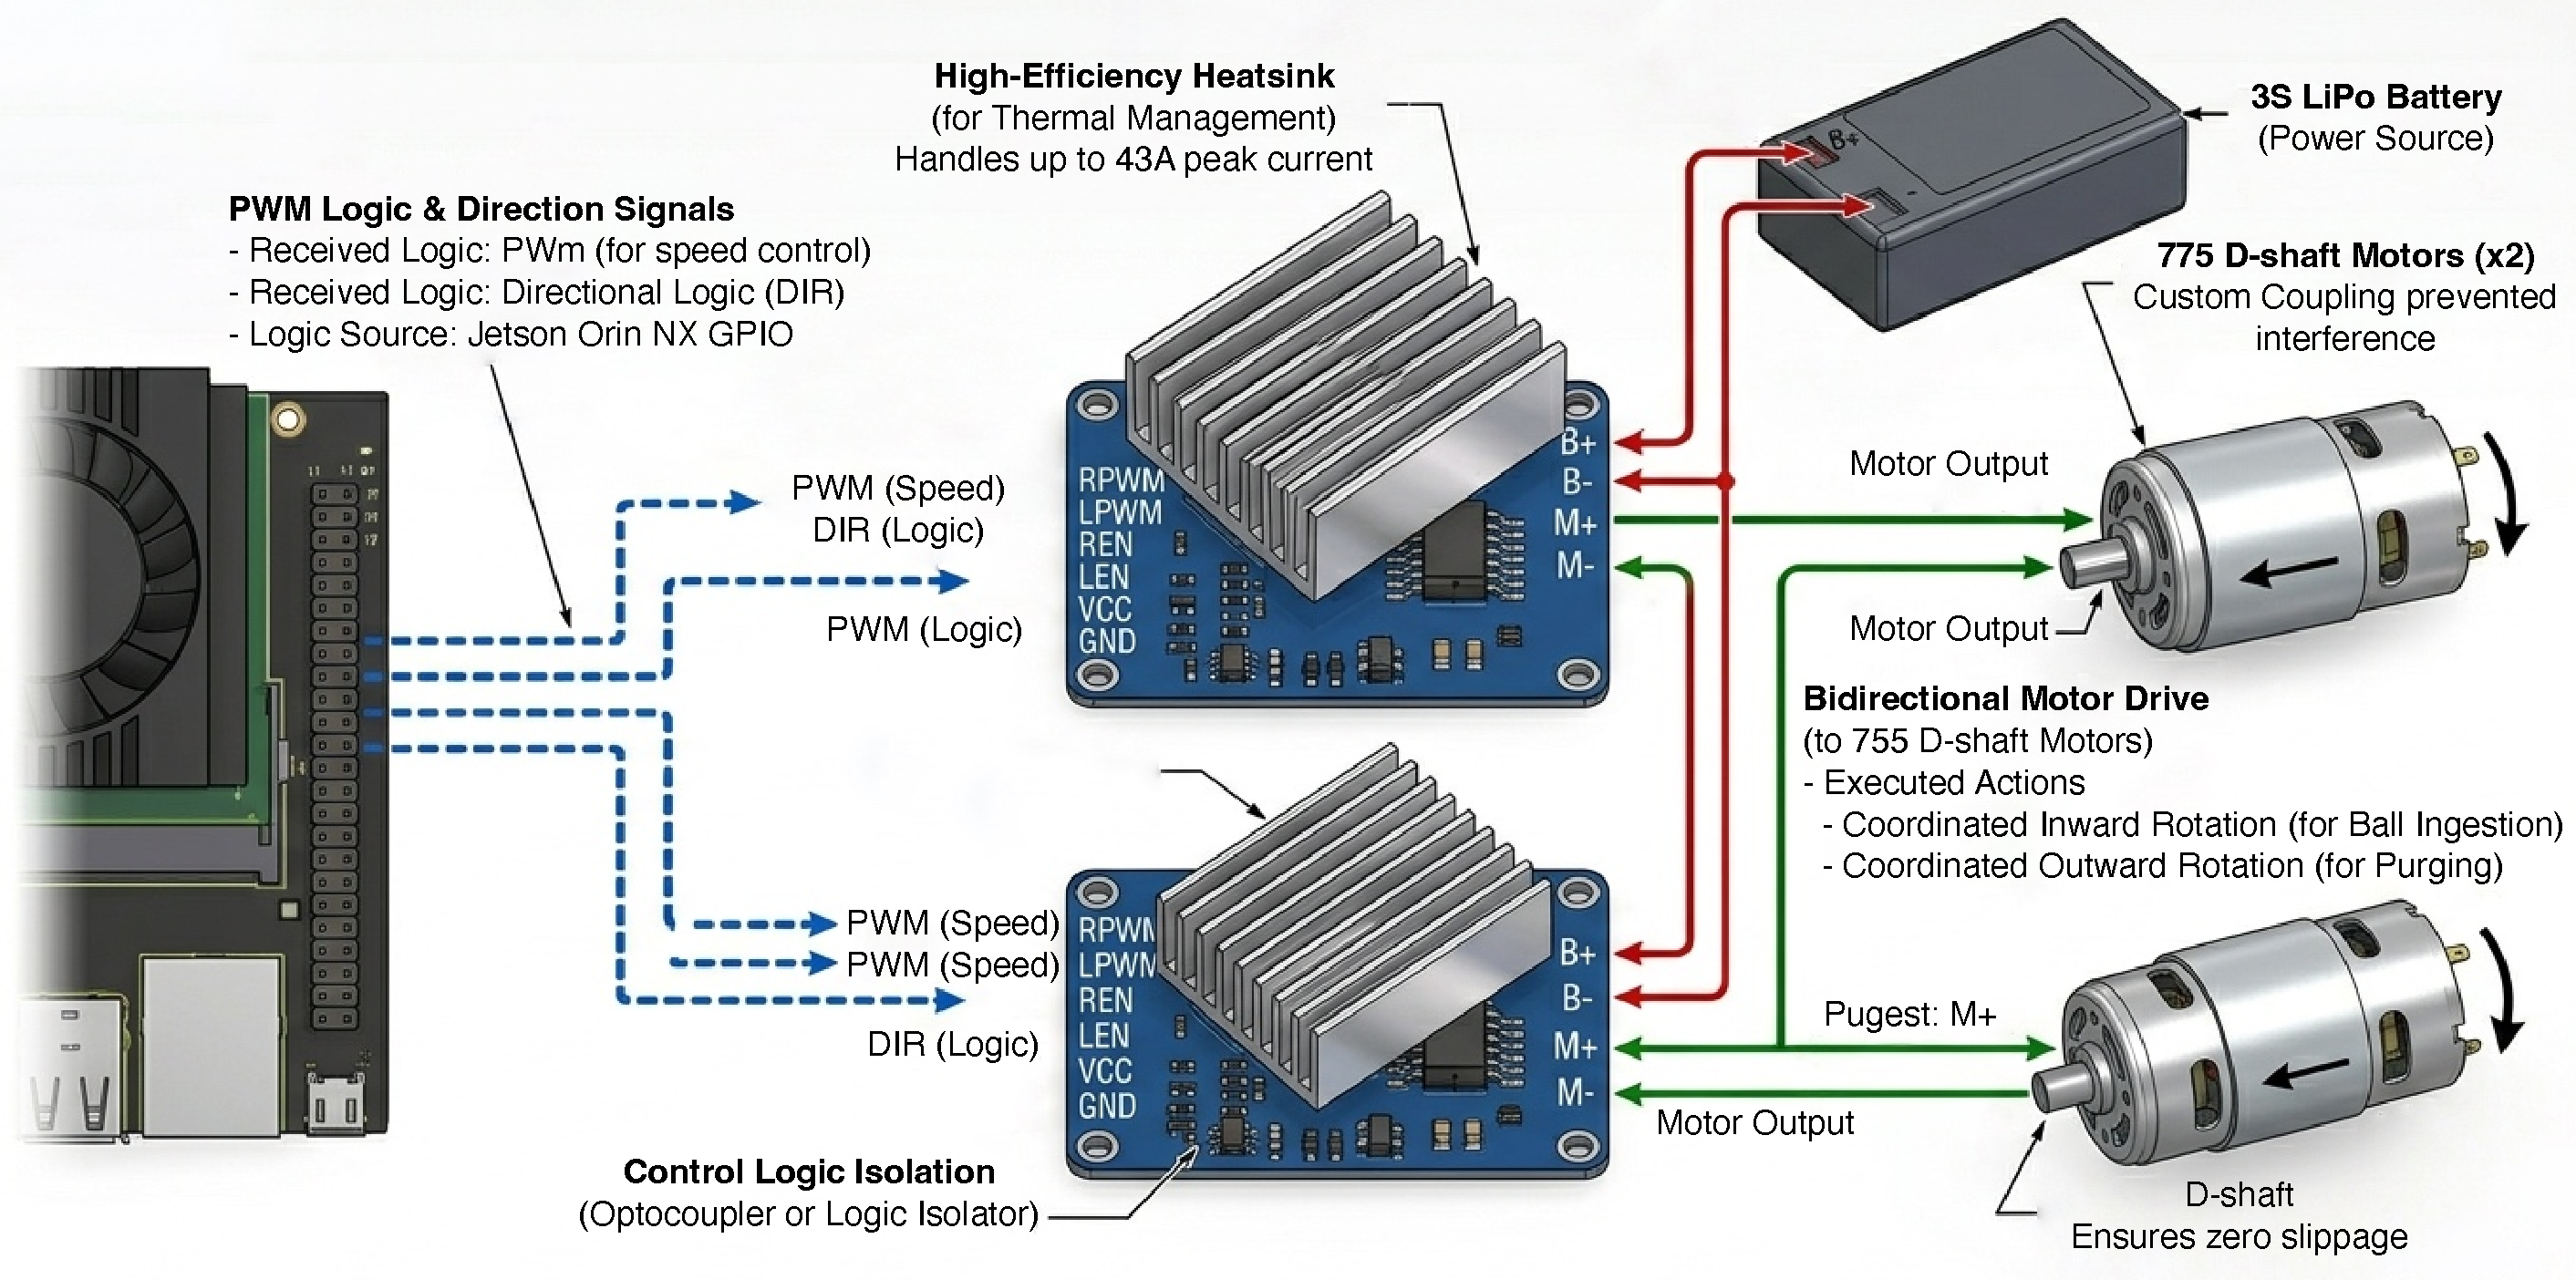
\includegraphics[width=0.7\textwidth]{figures/fig_drive.pdf}
  \caption{An engineering diagram detailing the BTS7960 high-current drive architecture for the CourtSweeper system, illustrating the connection of an NVIDIA Jetson Orin NX to two BTS7960 motor drivers powered by a 3S LiPo battery to control two 775 D-shaft motors, featuring logic signal connections, power distribution, bidirectional motor drive, and technical callouts for key components like heatsinks and motor features.}
  \label{fig_motor}
  \end{figure}


\subsection{Camera Setup}
\label{sec:camera}
The primary visual input via the integrated HD camera on the Robomaster EP chassis, which feeds raw video streams to the edge computing unit for target detection. The core hardware parameters of the integrated camera are detailed in Table \ref{tab:camera_specs}.

\begin{figure}[htbp]
  \centering
  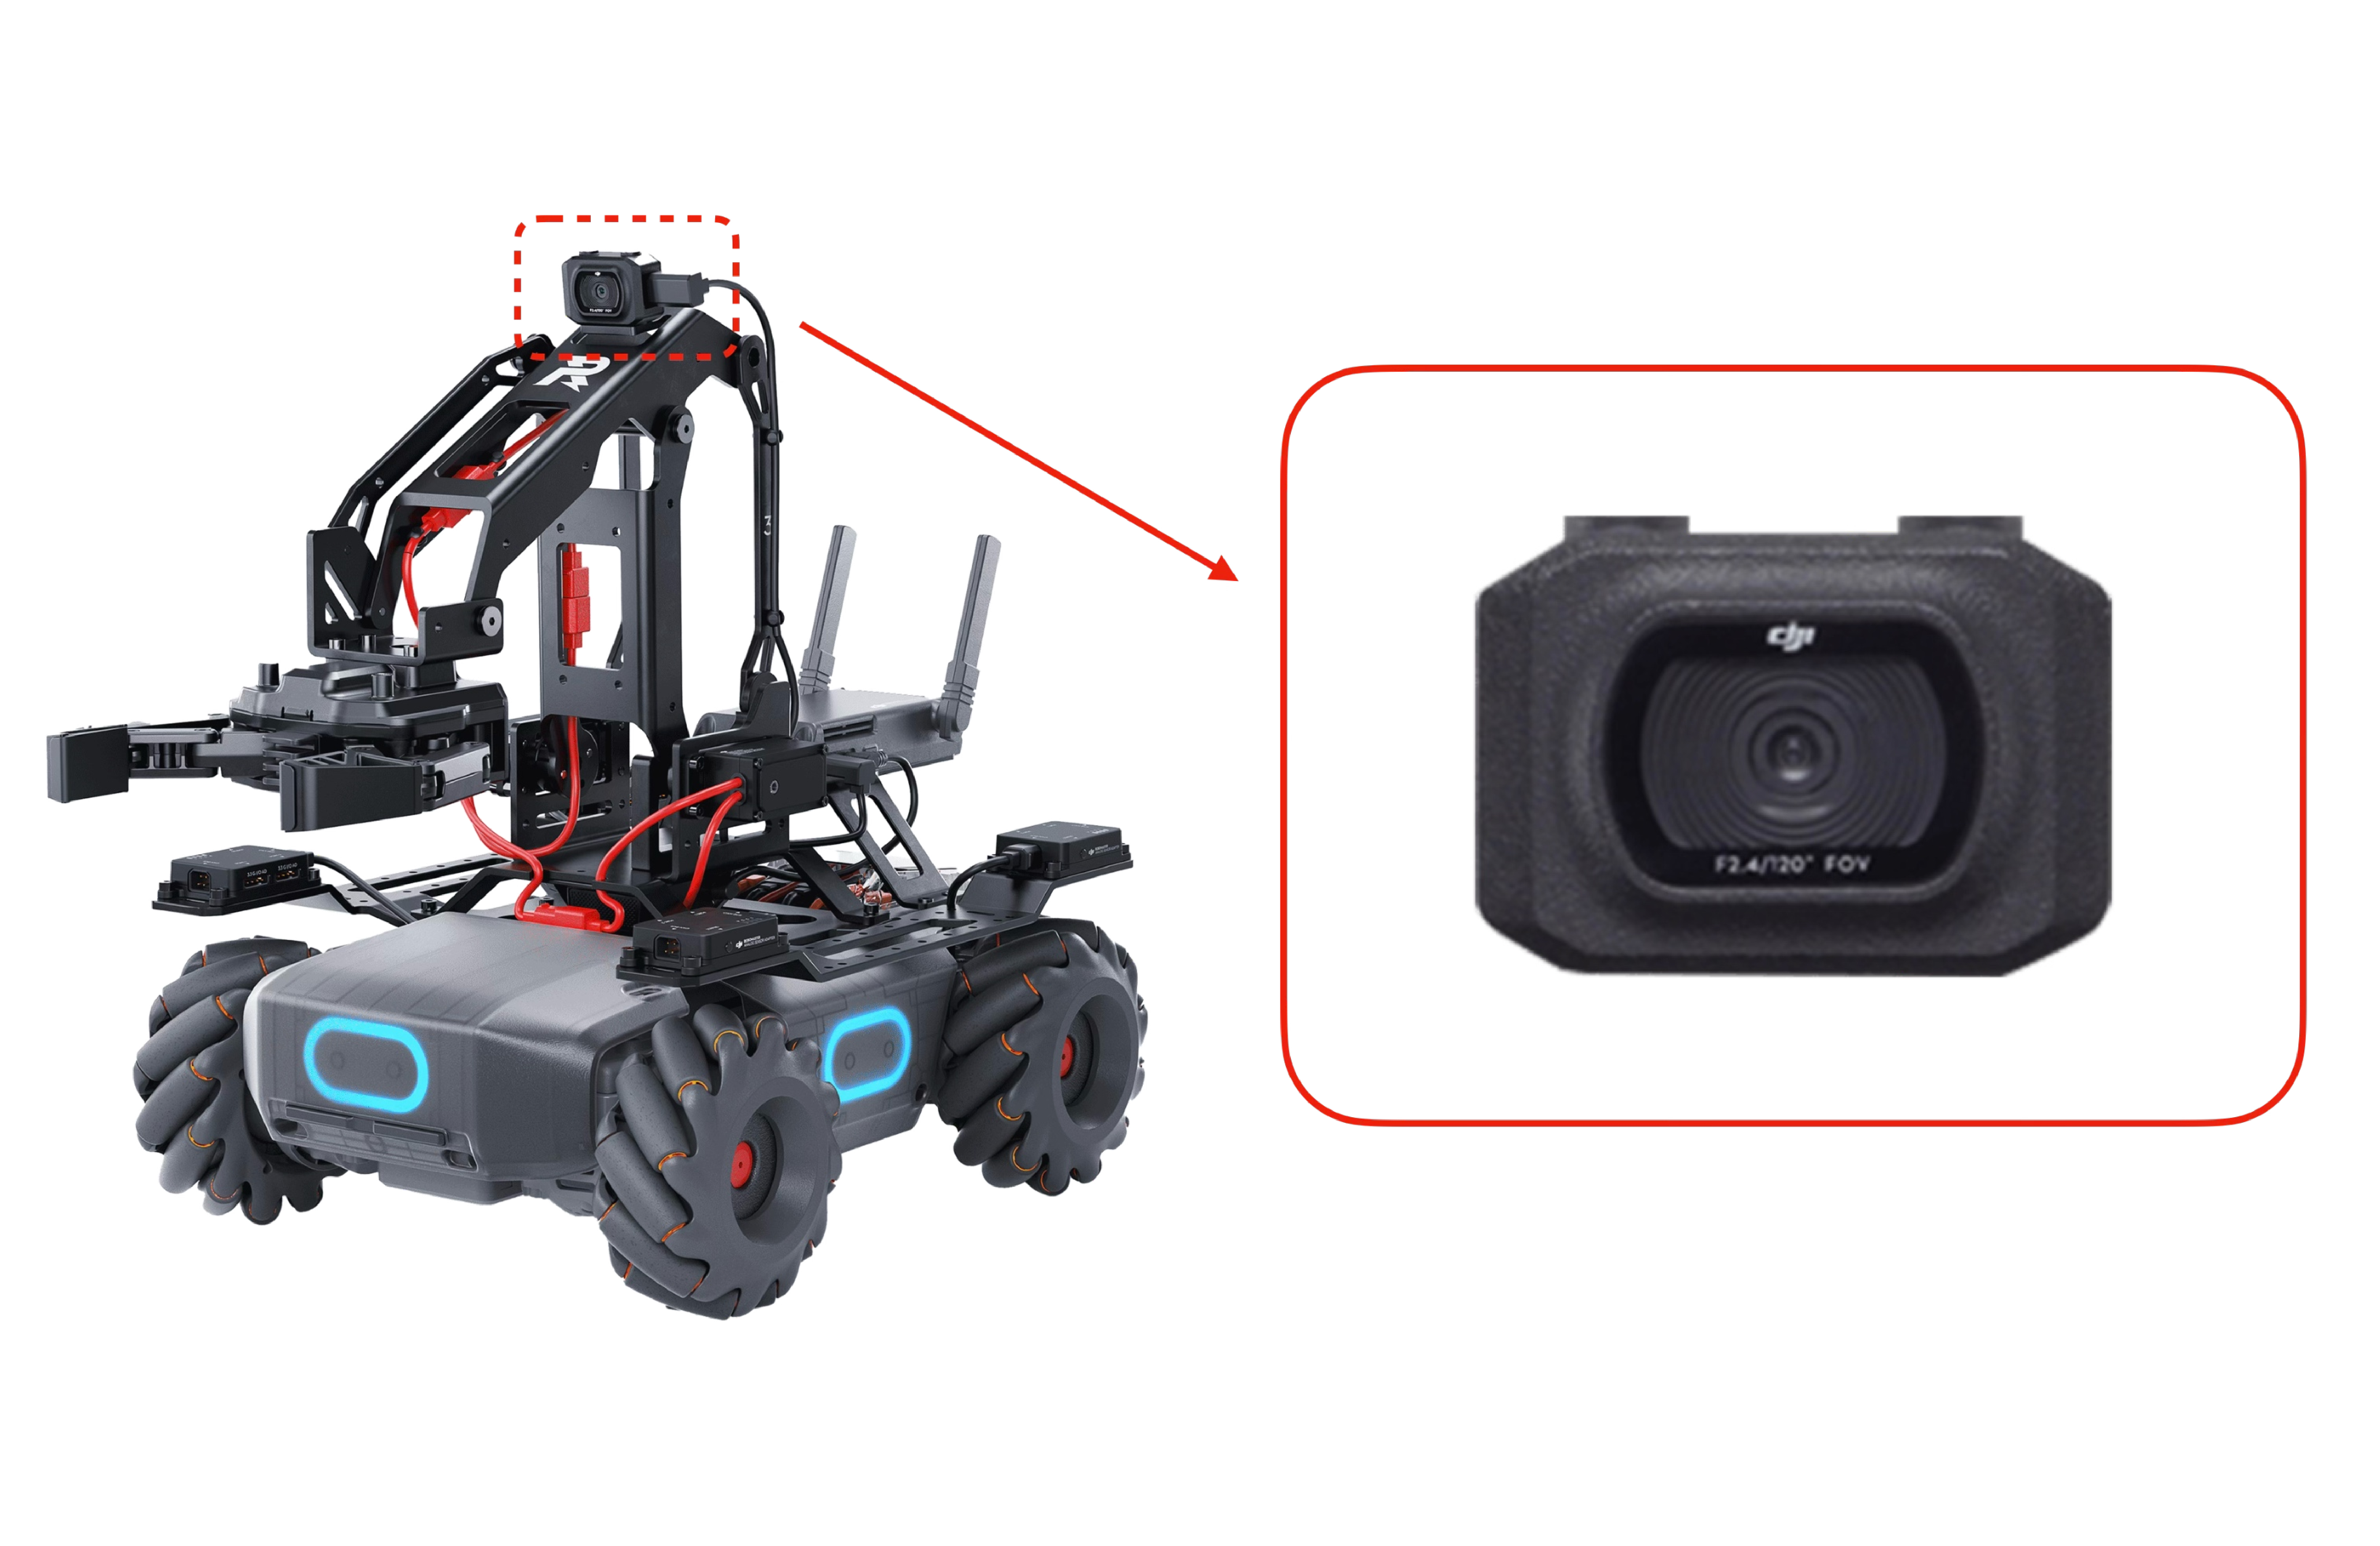
\includegraphics[width=0.65\textwidth]{figures/fig_camera.pdf}
  \caption{A physical picture of Robomaster EP Camera Module.}
  \label{fig_camera}
\end{figure}

\begin{table}[htbp]
  \footnotesize
  \centering
  \caption{DJI RoboMaster EP Integrated Camera Specifications}
  \label{tab:camera_specs}
  \renewcommand{\arraystretch}{1.2}
  \begin{tabular}{@{}ll@{}}
    \toprule
    \textbf{Hardware Parameter} & \textbf{Specification} \\
    \midrule
    \textbf{Sensor Type} & CMOS 1/4″, Effective Pixels: 5 MP \\
    \textbf{Field of View (FOV)} & 120$^\circ$ \\
    \textbf{Max Video Resolution} & FHD: 1080p@30fps / HD: 720p@30fps \\
    \textbf{Max Video Bitrate} & 16 Mbps \\
    \textbf{Max Still Photo Resolution} & 2560 $\times$ 1440 \\
    \bottomrule
  \end{tabular}
\end{table}


\subsection{DJI RoboMaster EP Chassis}
\label{sec:dji_chassis}

\begin{figure}[htbp]
  \centering
  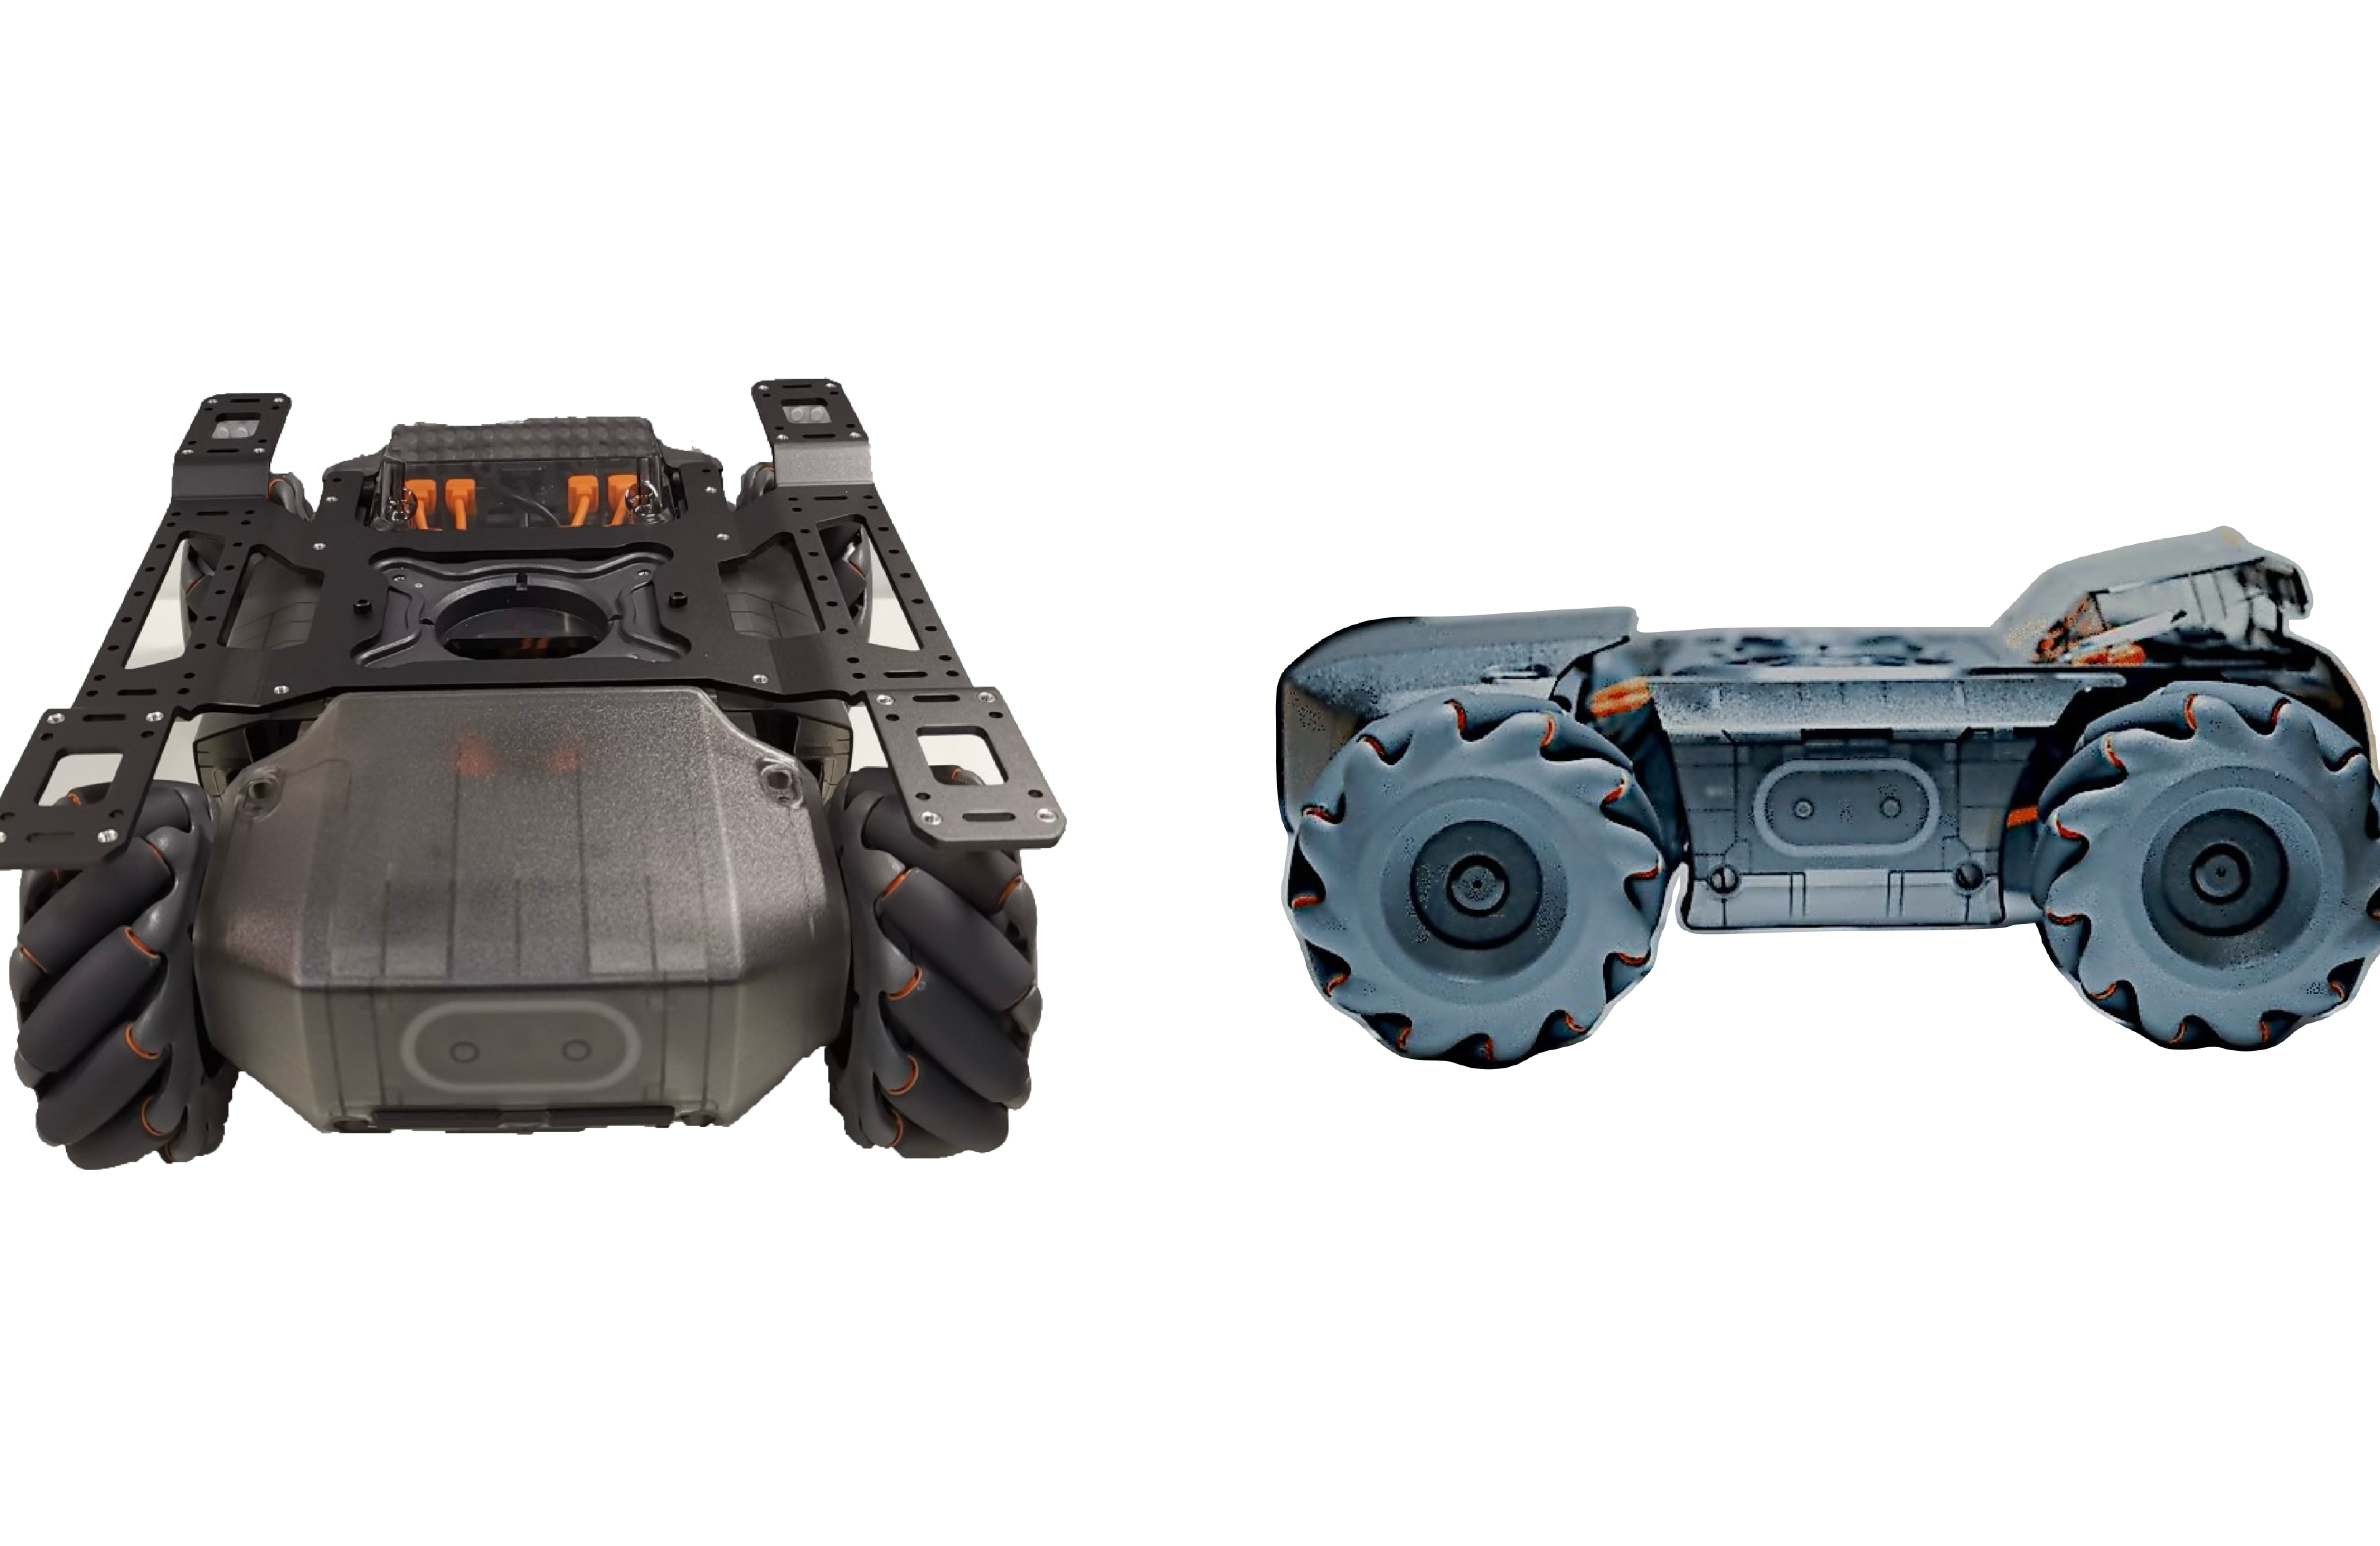
\includegraphics[width=0.65\textwidth]{figures/fig_chassis.pdf}
  \caption{A physical picture of Robomaster EP Chassis Module.}
  \label{fig_chassis}
\end{figure}

The foundation of the CourtSweeper is the DJI RoboMaster EP chassis. Selected for its industrial-grade stability and payload capacity, the chassis is equipped with four Mecanum wheels, granting the robot true omnidirectional mobility. This holonomic drive system is crucial for the precise spatial adjustments required to align the front-facing intake mechanism with scattered tennis balls without needing a turning radius. 


\subsection{Custom Intake Mechanism}
\label{sec:intake_mech}

To achieve reliable and rapid ball collection, a custom dual-roller intake mechanism~\cite{dual_roller} was designed and mounted at the front of the chassis. The actuation is driven by two high-torque 775 DC motors (D-shaft configuration, rated at 12V and 4600 RPM).

\begin{figure}[htbp]
  \centering
  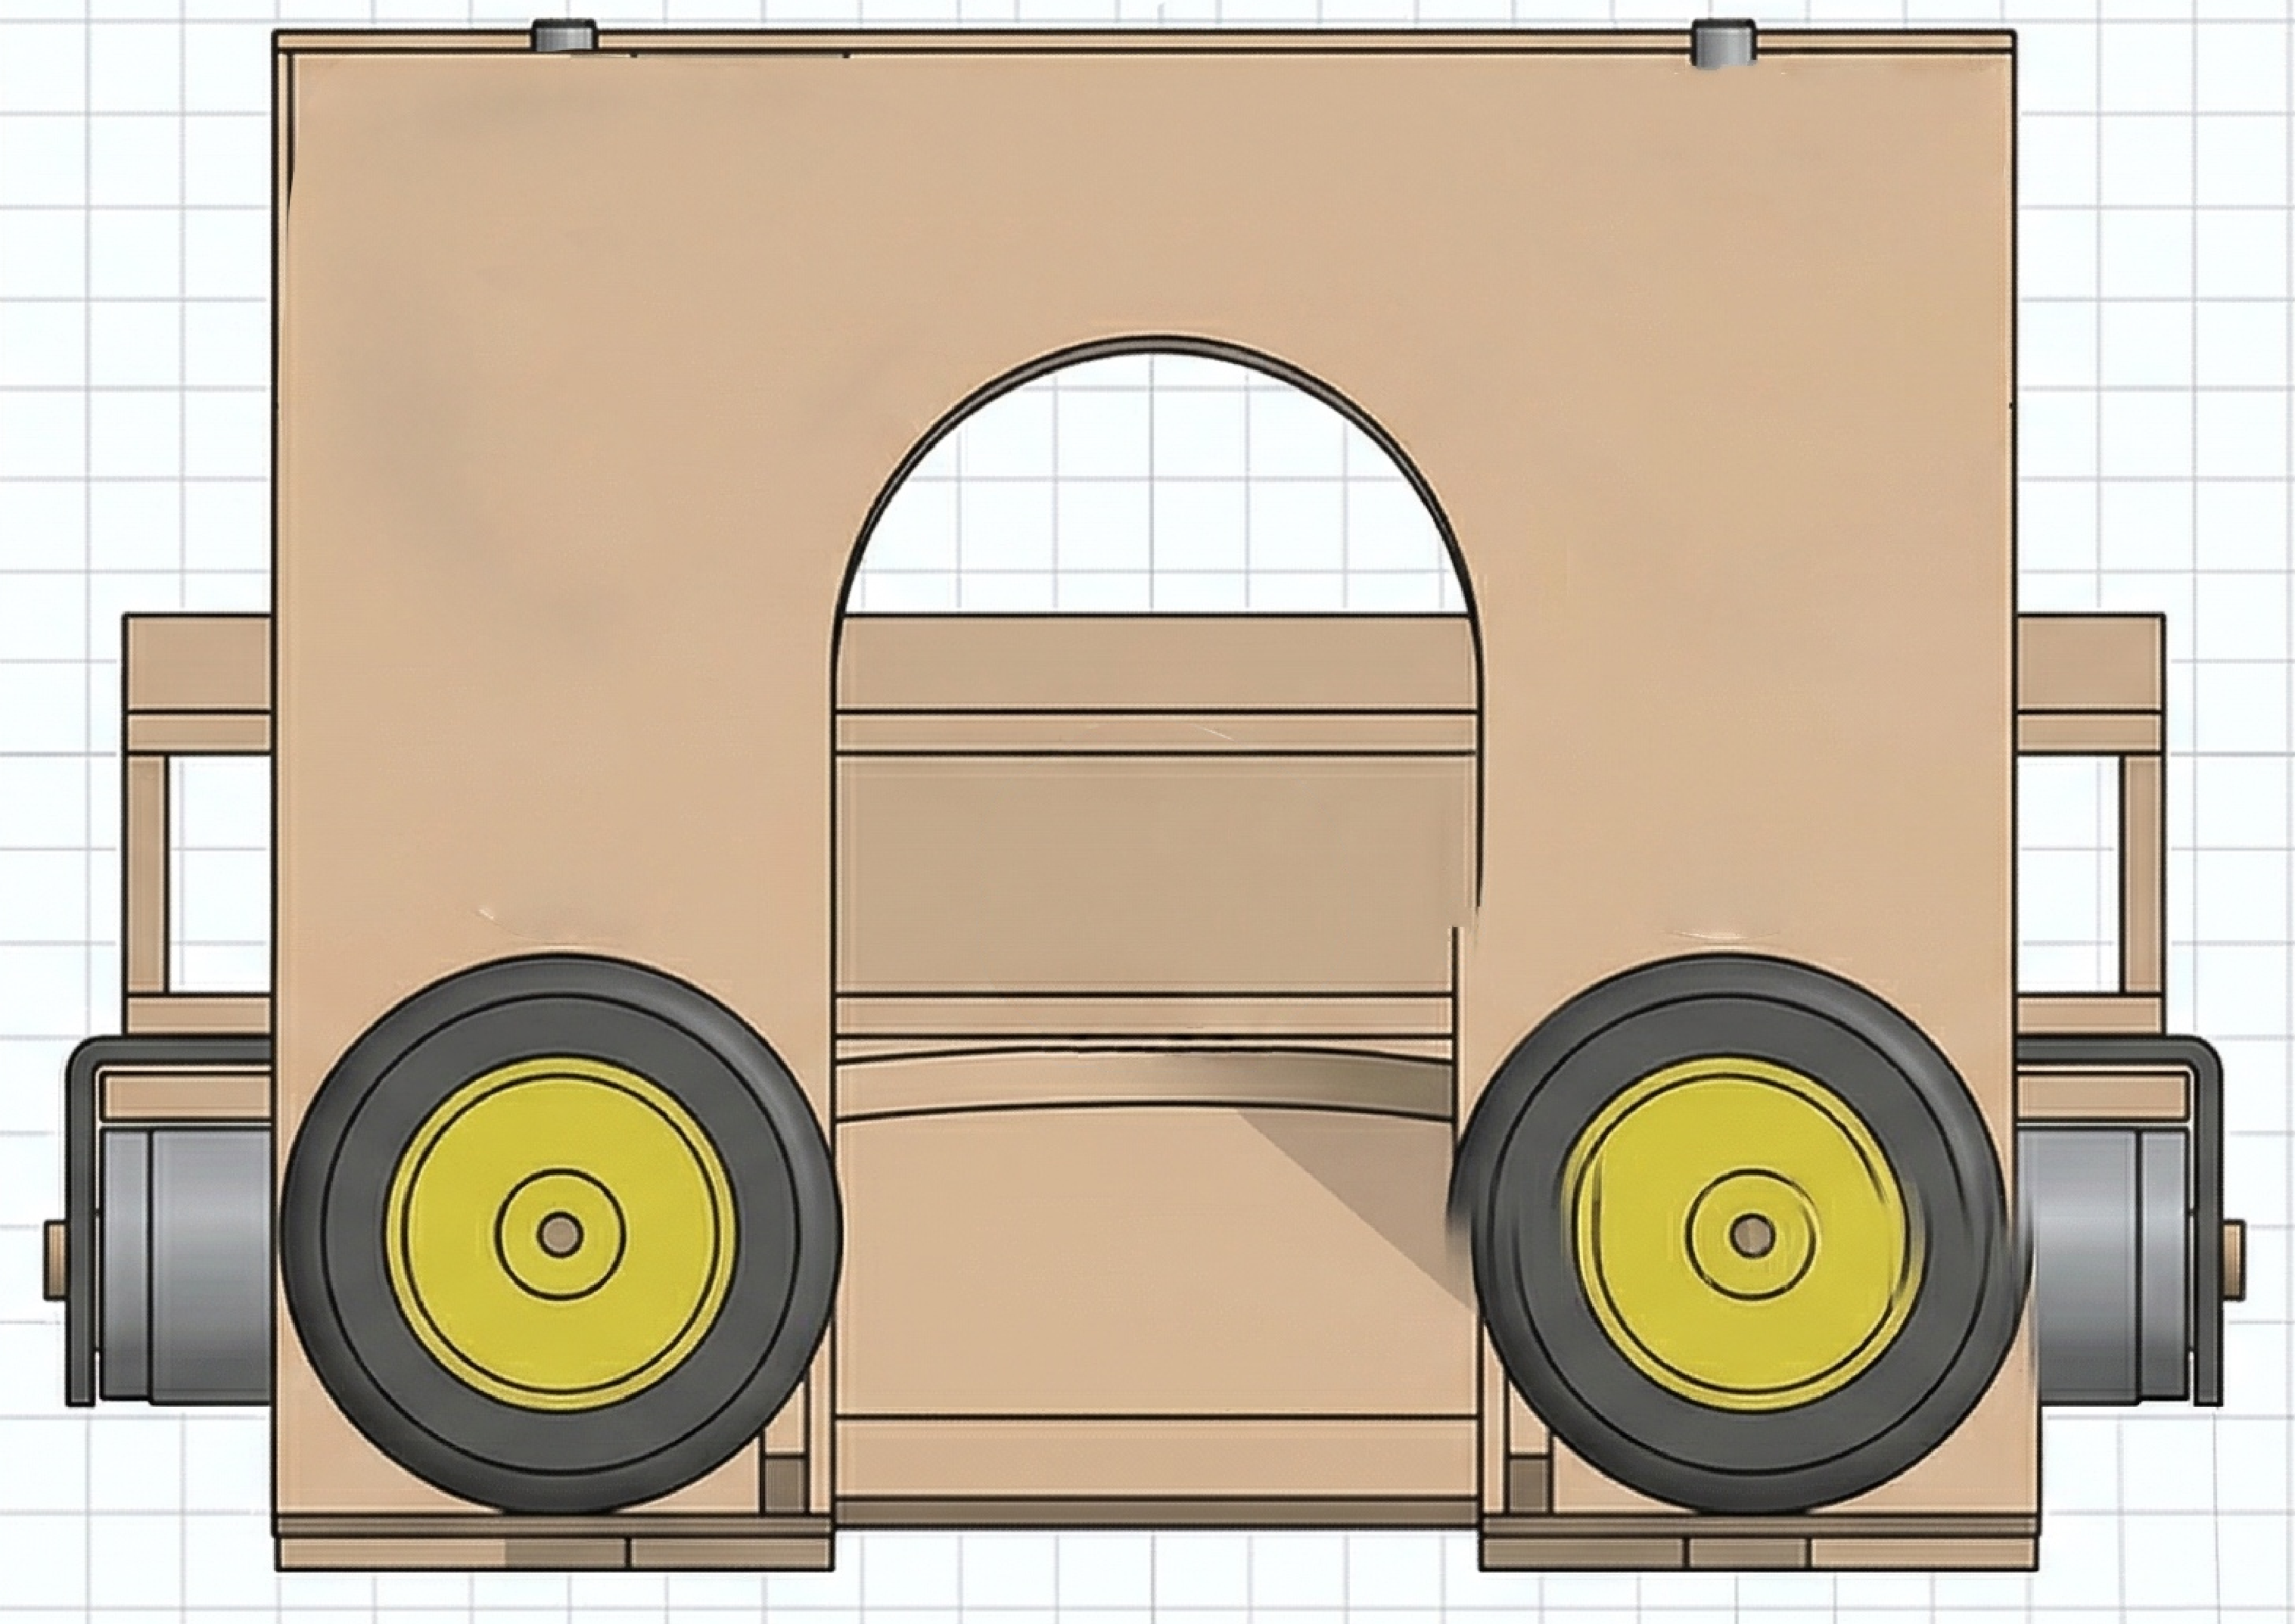
\includegraphics[width=0.45\textwidth]{figures/fig_dual_roller.pdf}
  \caption{A detailed front-on view of the Courtsweeper dual-roller intake mechanism.}
  \label{fig_roller_mech}
\end{figure}

\begin{itemize}
  \item \textbf{Mechanical Coupling:} The motors are mated to 60mm solid rubber wheels featuring high-friction hexagonal grooves via 30mm extended brass couplings. This extended design provides essential clearance to prevent mechanical interference between the rotating wheel hubs and the motor casing, while the D-shaft ensures zero slippage under high torque.

  \item \textbf{Motor Drivers:} Two BTS7960 high-current motor driver modules (capable of handling up to 43A peak current) are utilized to independently control the two motors. They receive Pulse Width Modulation (PWM) and directional logic signals from the central computing unit to execute coordinated inward rotation (for ball ingestion) or outward rotation (for purging).
\end{itemize}

\begin{figure}[htbp]
  \centering
  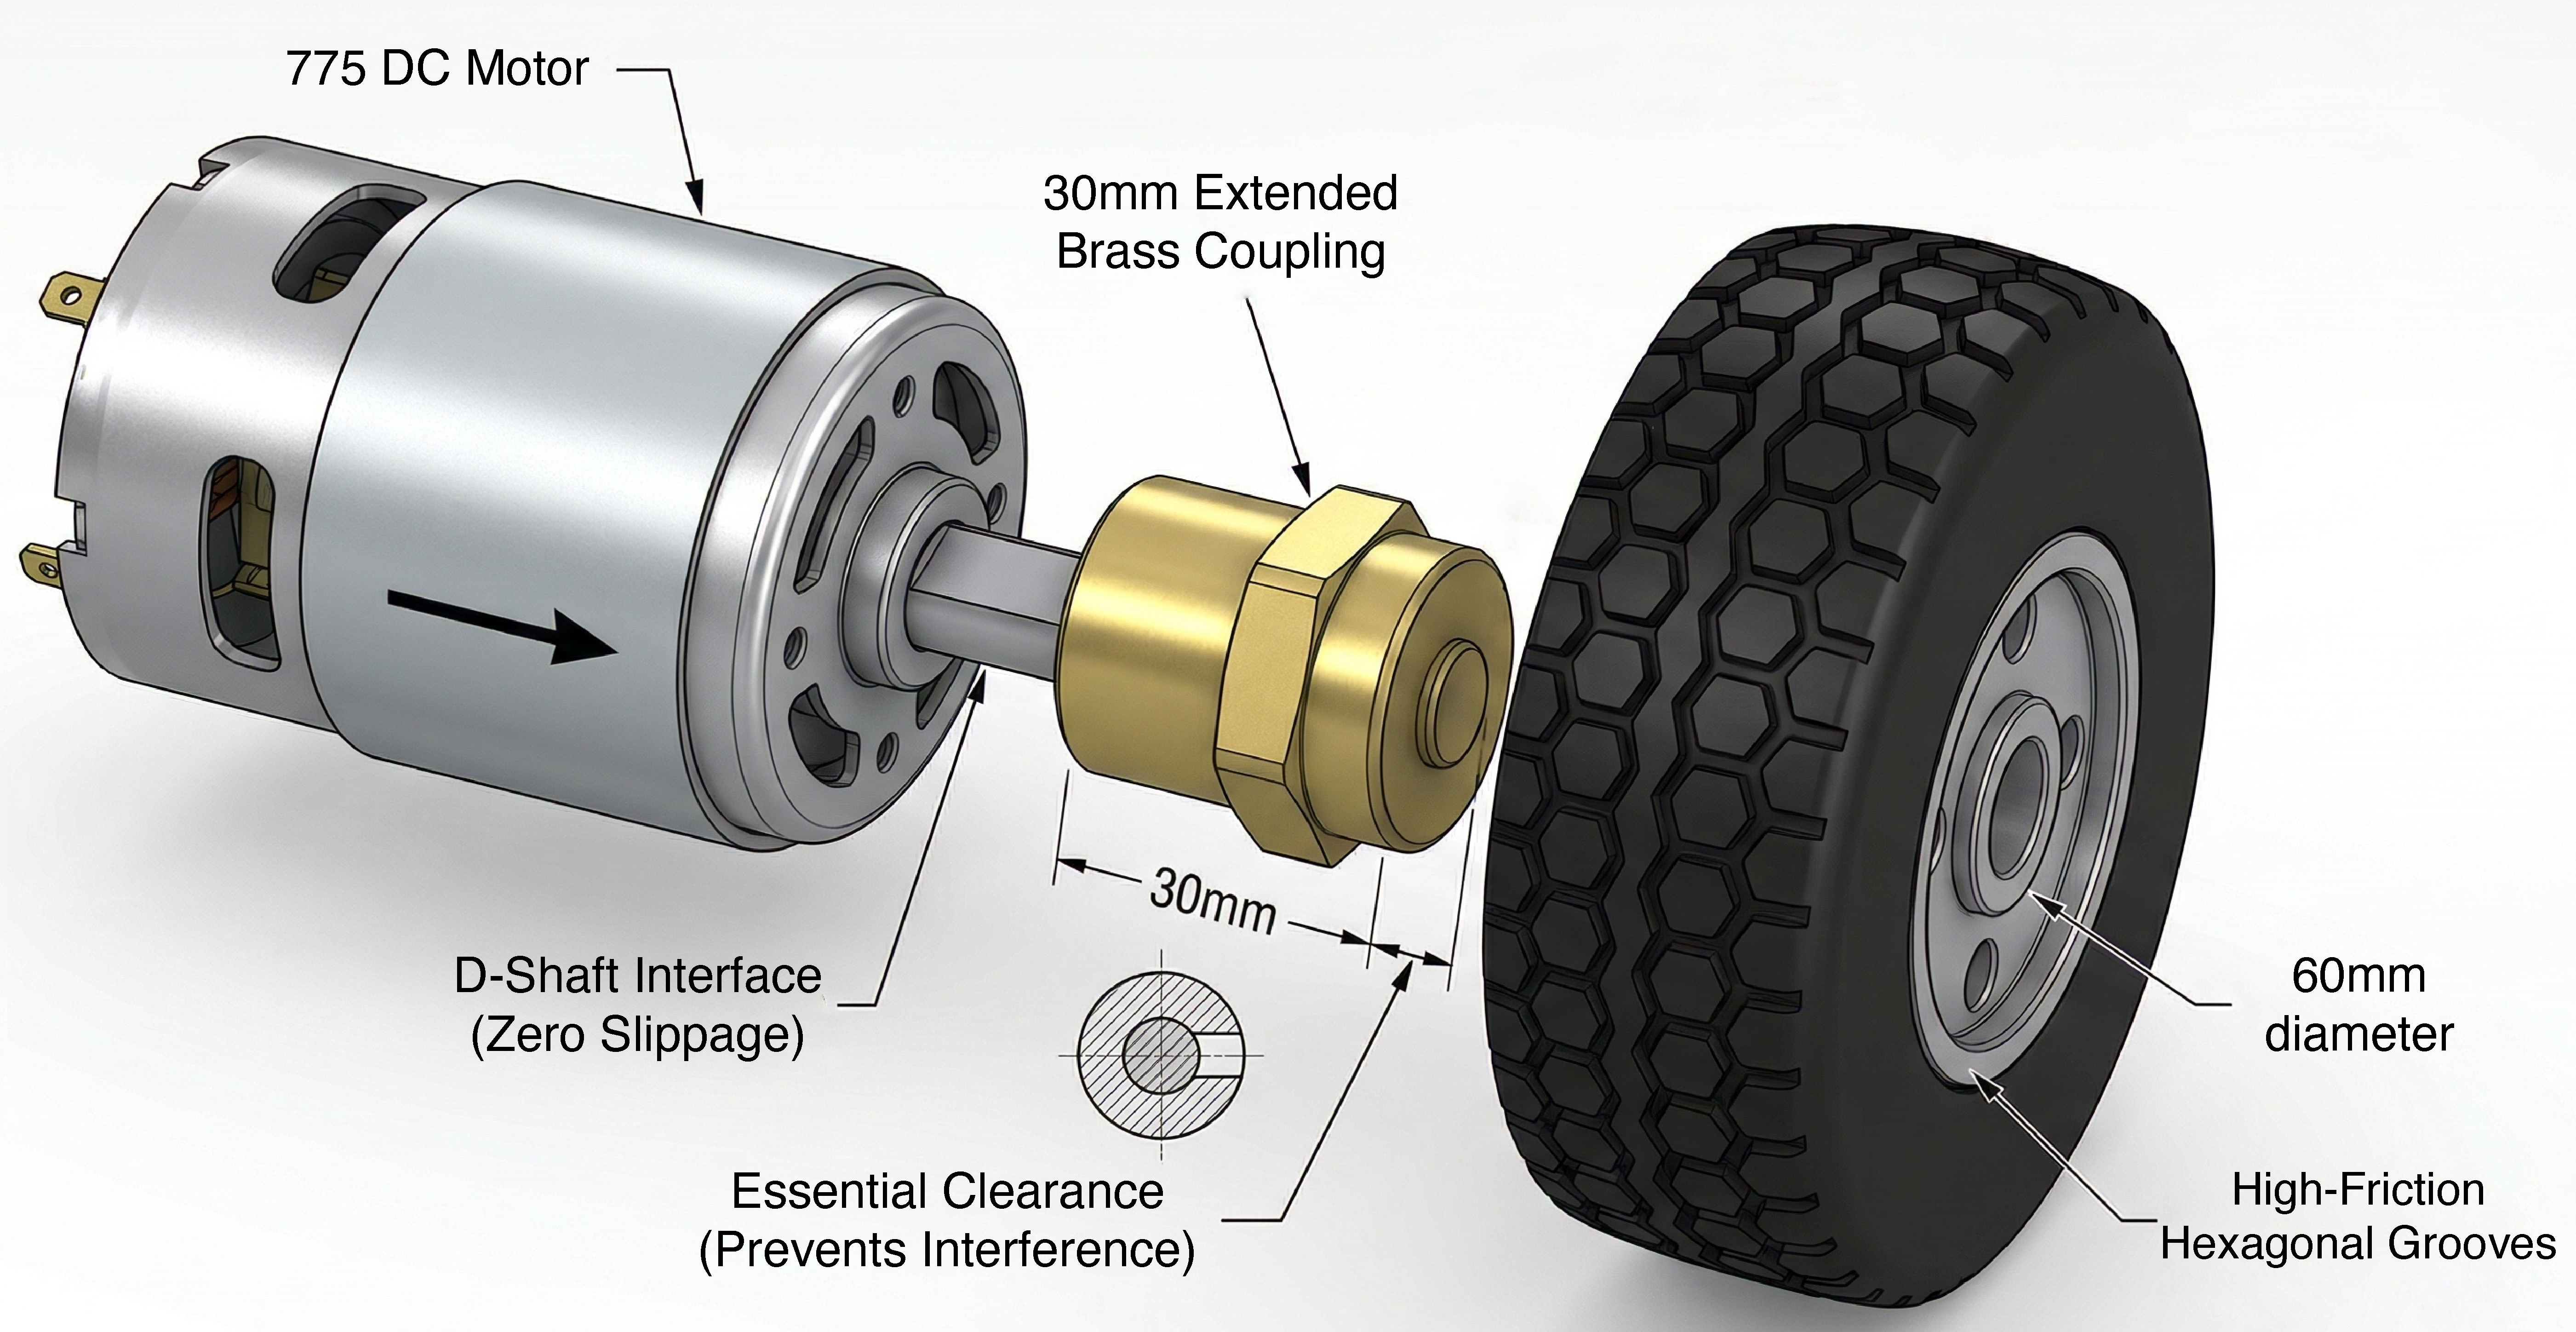
\includegraphics[width=0.7\textwidth]{figures/fig_motor.pdf}
  \caption{Close-up view of the mechanical coupling. The 30mm extended brass coupling provides critical operational clearance between the 775 motor casing and the high-friction intake roller.}
  \label{fig_motor}
\end{figure}


\subsection{LiDAR Sensor Setup}
\label{sec:lidar}
To ensure precise operational boundary gridding and efficient path planning (as outlined in the software architecture~Fig.\ref{fig_software_overview}), the Courtsweeper incorporates a dedicated 2D LiDAR sensor. Based on a triangulation principle, this sensor provides robust 2D scanning of the court environment and potential obstacles.

\begin{itemize}
  \item \textbf{Sensor Details:} The selected hardware is the YDLIDAR X3-YB-1 triangulation-based LiDAR. It is mounted at the rear of the chassis and interfaces with the Jetson Orin NX via a customized USB-serial connection.
  \item \textbf{Specifications:} The X3-YB-1 offers a maximum distance range of up to 10 meters, enabling comprehensive court coverage. Key operational parameters include a sampling frequency of 4000 Hz, a standard rotating frequency of 7 Hz, and an angular resolution of 0.6$^\circ$.
\end{itemize}

\begin{figure}[htbp]
  \centering
  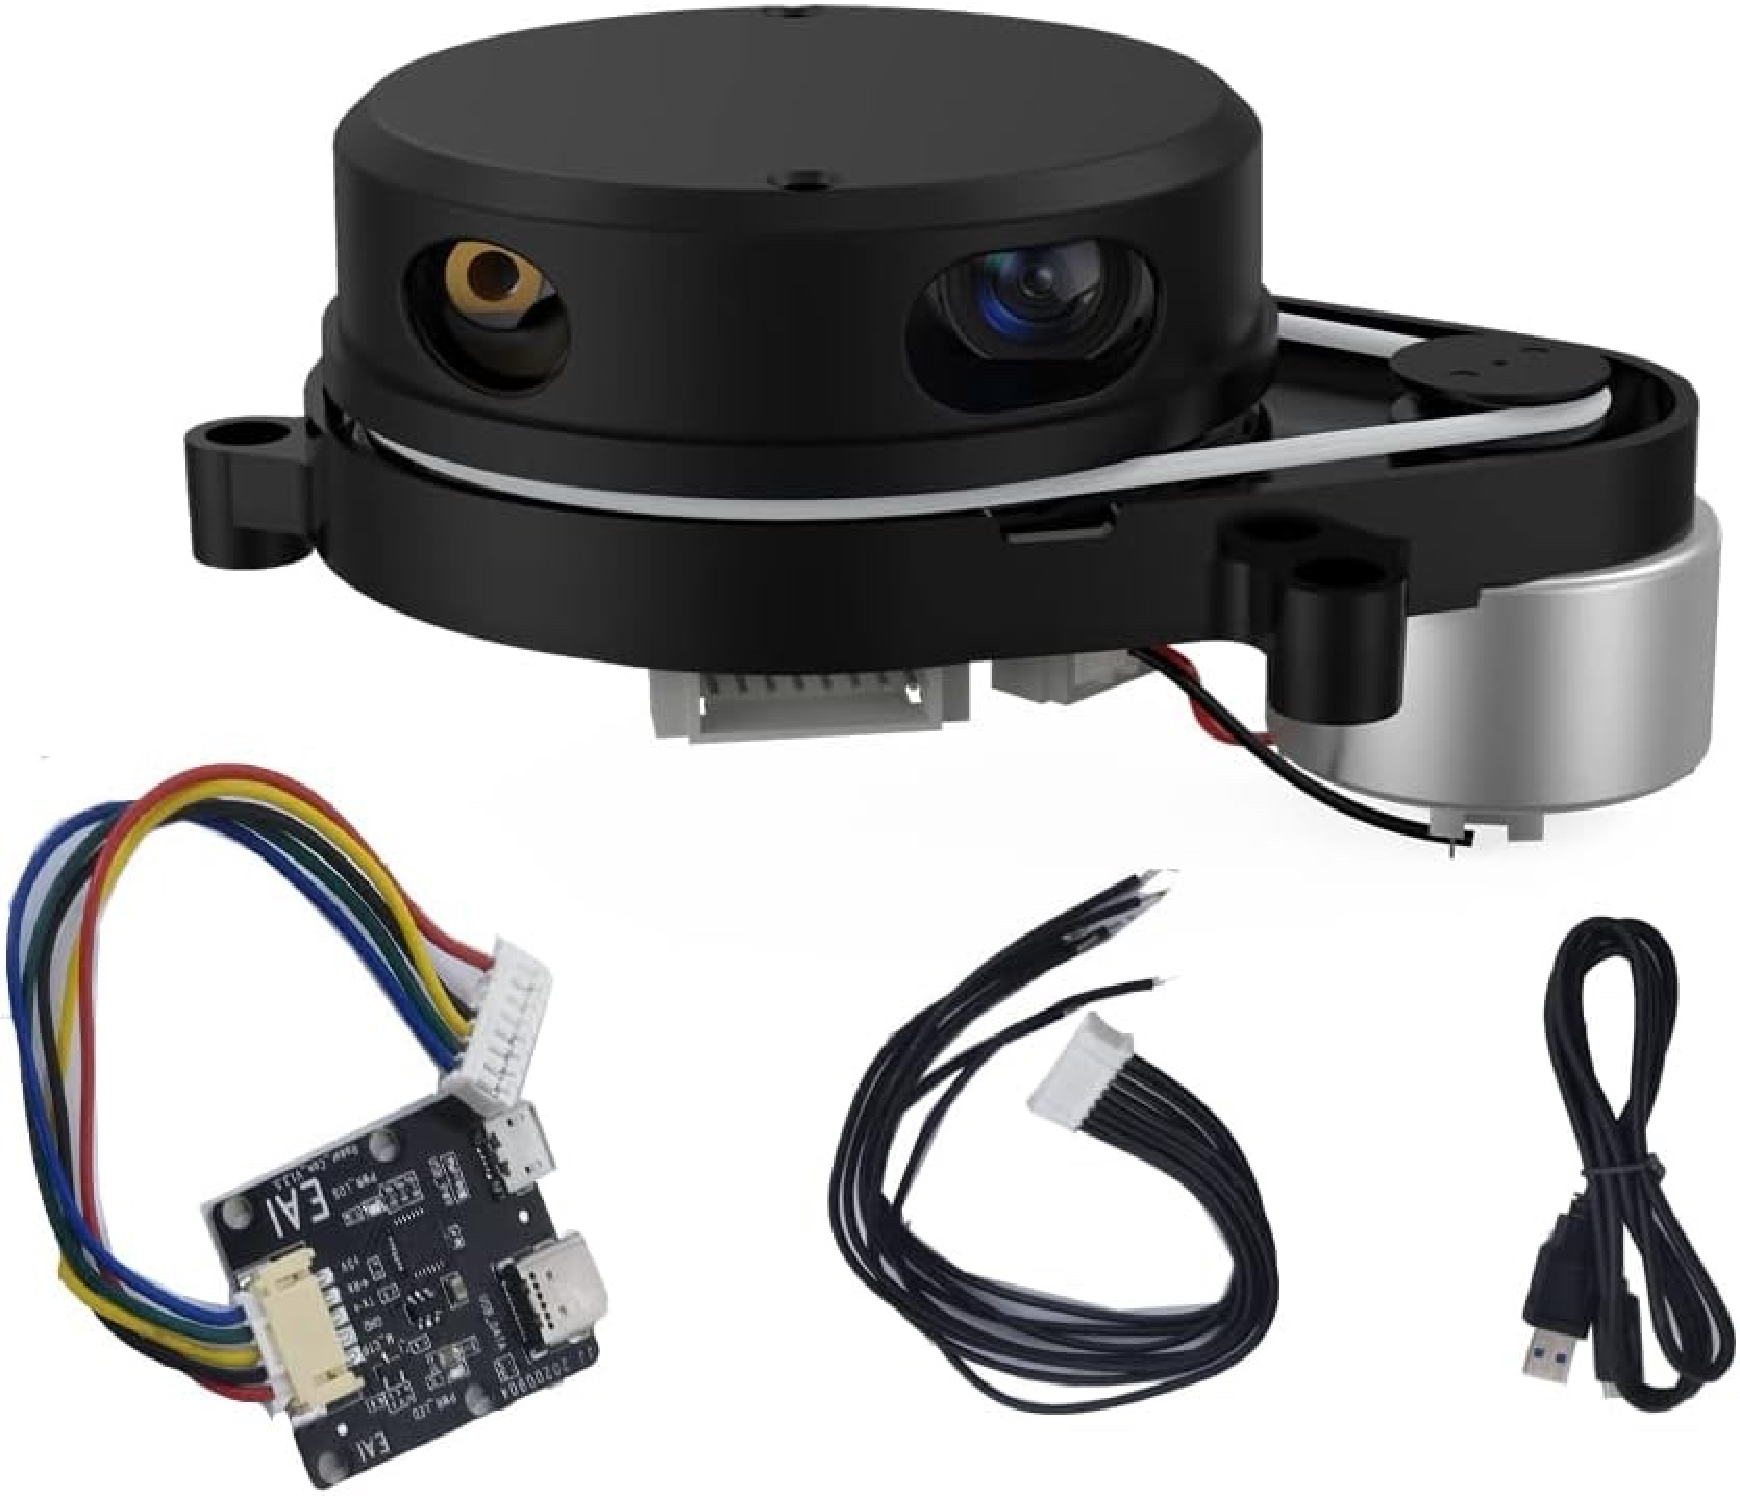
\includegraphics[width=0.4\textwidth]{figures/fig_lidar.pdf}
  \caption{A physical picture of the YDLIDAR X3-YB-1 LiDAR sensor.}
  \label{fig_lidar}
\end{figure}


\subsection{Jetson Orin NX Setup}
\label{sec:jetson_setup}
The cognitive core of the system is the NVIDIA Jetson Orin NX. Acting as the Edge Computing Unit, it is responsible for handling computationally intensive tasks locally, thereby eliminating cloud-dependency and minimizing latency. The Jetson module runs the Ubuntu operating system and is configured to:
\begin{enumerate}
  \item Execute the YOLO object detection pipeline concurrently with OpenCV operations to process the H.264 video stream captured by the DJI chassis.
  \item Run the customized RoboMaster-SDK-Ultra to translate bounding box coordinates into proportional navigation commands.
  \item Generate precise PWM signals via its GPIO pins to command the BTS7960 drivers.
  \item Operate in Access Point (AP) mode to establish a localized Wi-Fi network for the iOS UI client.
\end{enumerate}

\begin{figure}[htbp]
  \centering
  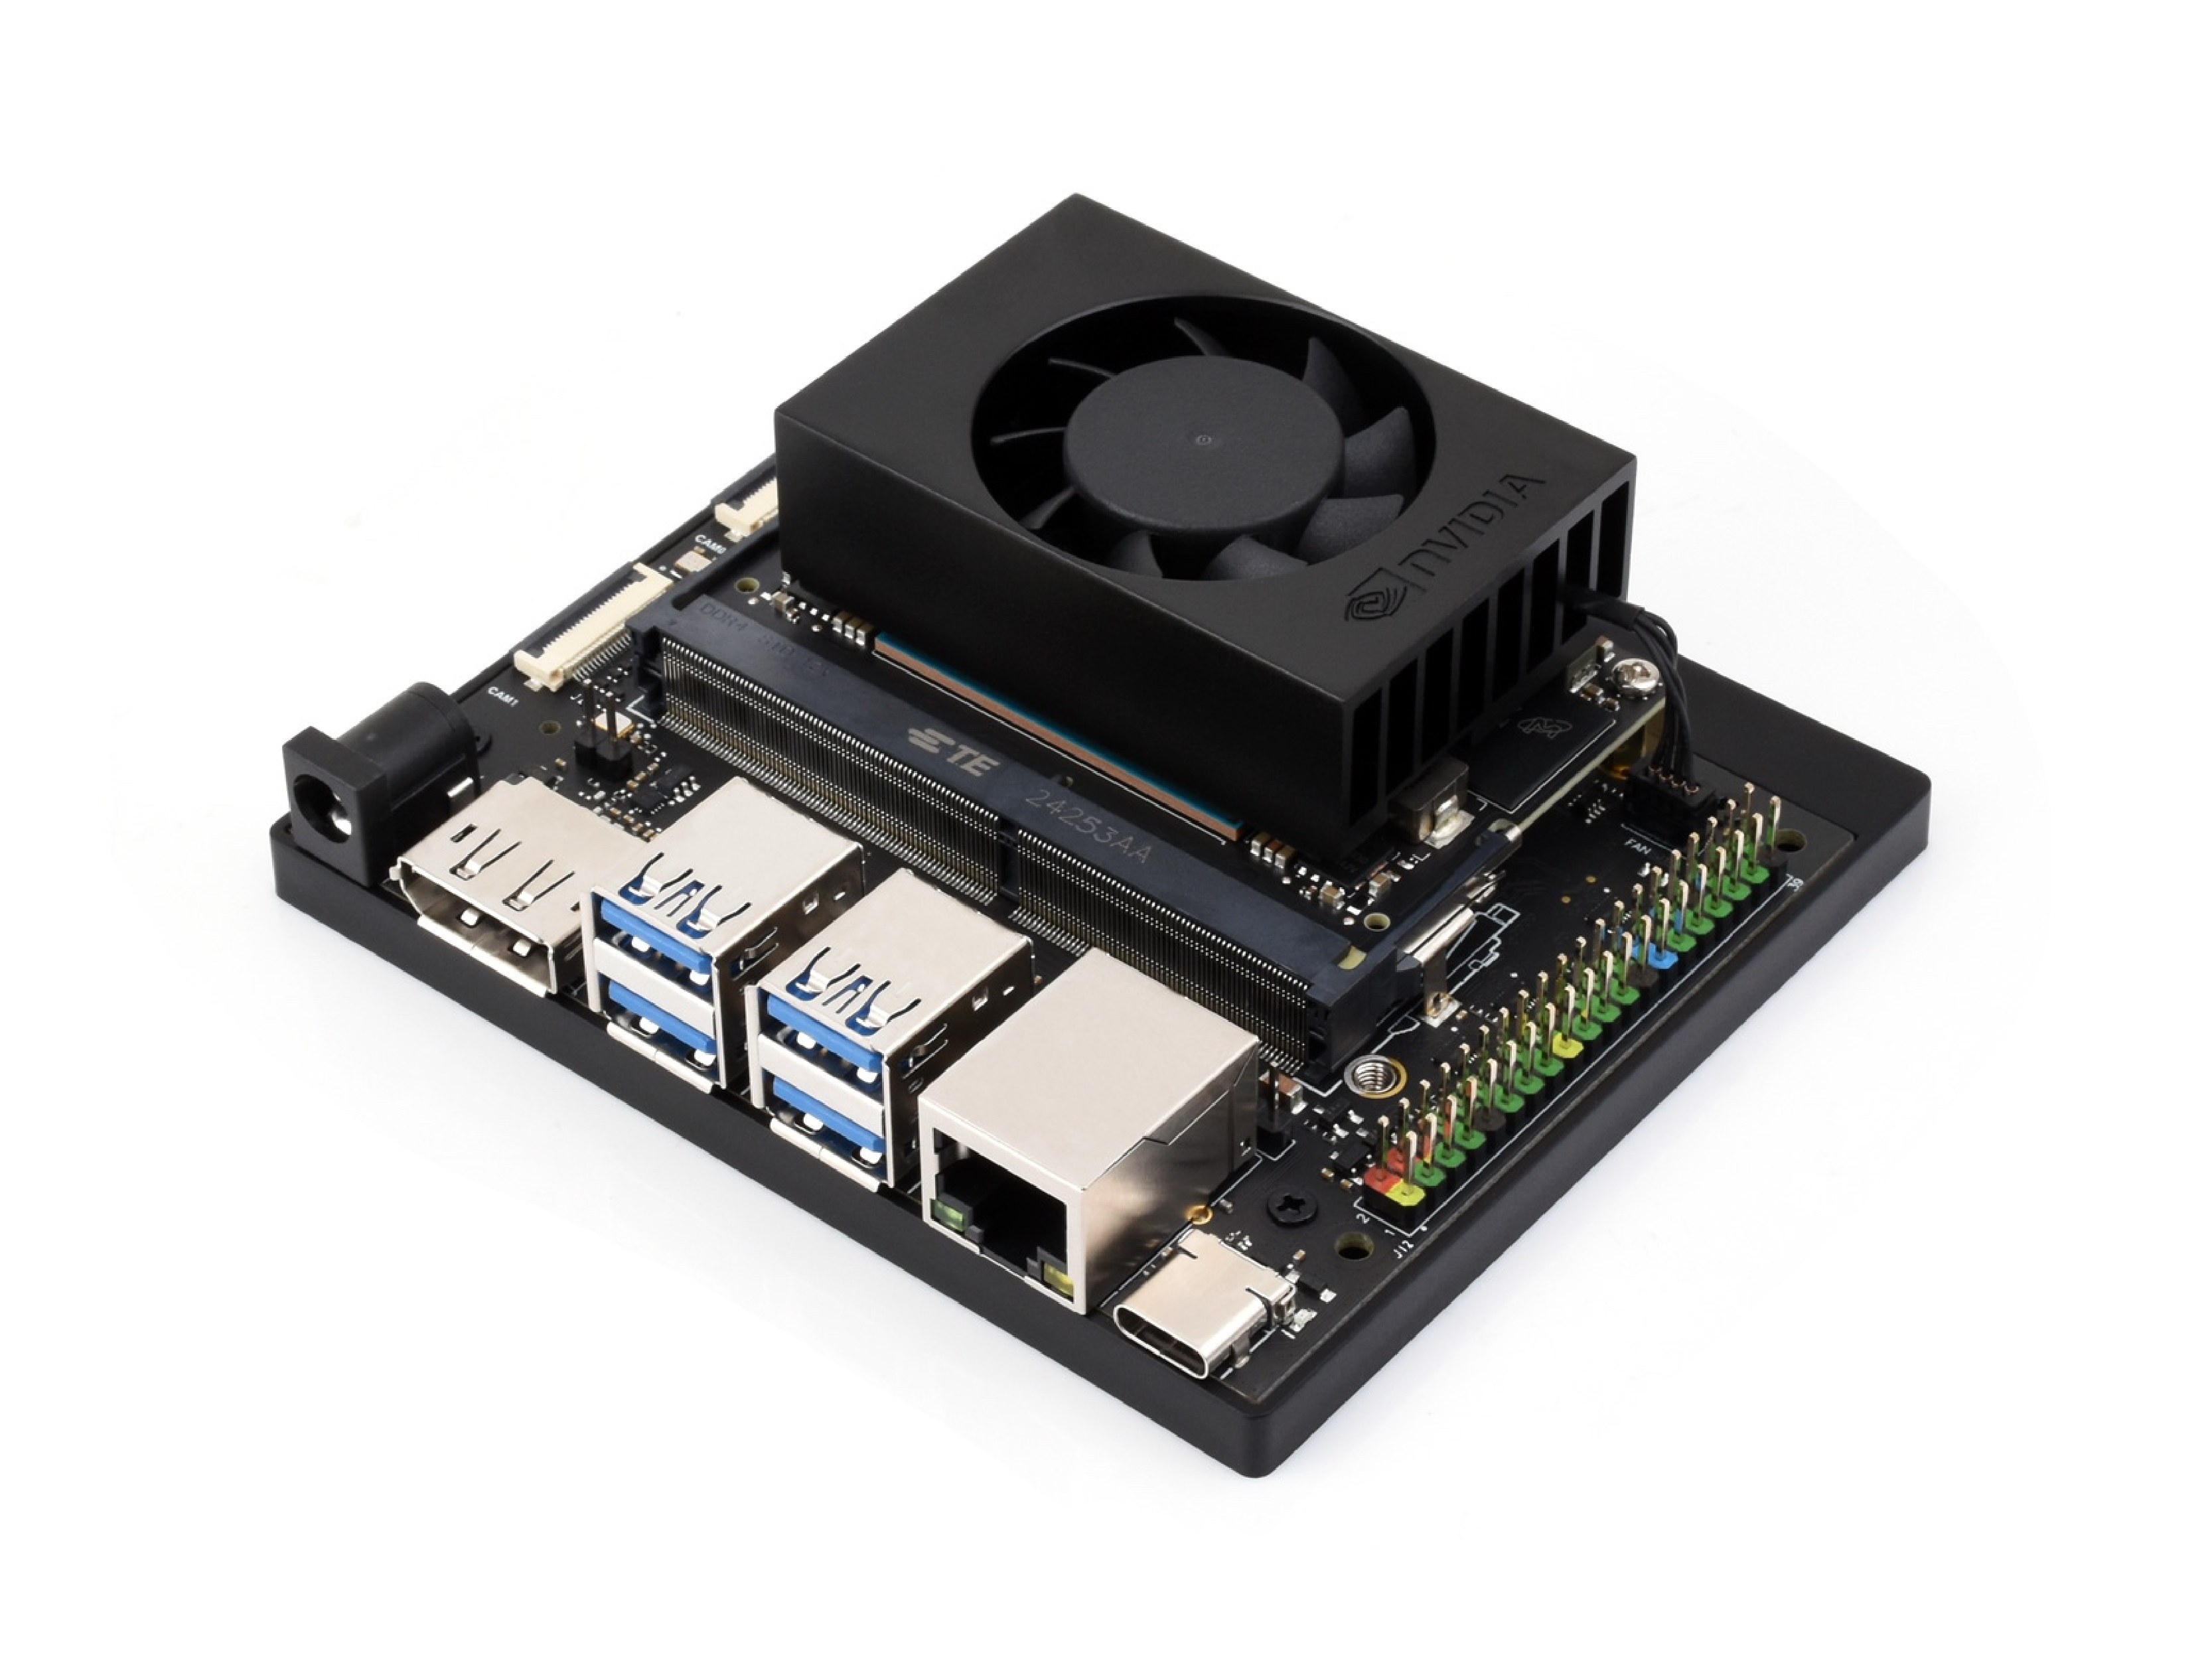
\includegraphics[width=0.55\textwidth]{figures/fig_jetson.pdf}
  \caption{A physical picture of NVIDIA jetson Orin NX.}
  \label{fig_jetson}
\end{figure}


\subsection{Power Management System}
\label{sec:power_sys}
Given the diverse voltage requirements and the risk of electromagnetic interference from high-current motors, the CourtSweeper employs an isolated, multi-rail power distribution topology:
\begin{itemize}
  \item \textbf{Mobility Power:} The DJI RoboMaster EP chassis and its onboard camera are powered autonomously by the proprietary DJI Intelligent Battery (3S LiPo, Nominal 10.8V, 2400mAh, 25.92Wh).

  \item \textbf{Actuation Power:} The 775 intake motors and BTS7960 drivers are powered by a dedicated 3S (11.1V) Lithium Polymer (LiPo) battery rated at 5200mAh and 40C discharge. This ensures the motors receive sufficient burst current during ball compression without inducing voltage sags in the logic circuits. A low-voltage buzzer (BX100) is attached to the balance lead for real-time cell monitoring.
  
  \begin{figure}[htbp]
    \centering
    \begin{minipage}{0.48\textwidth}
      \centering
      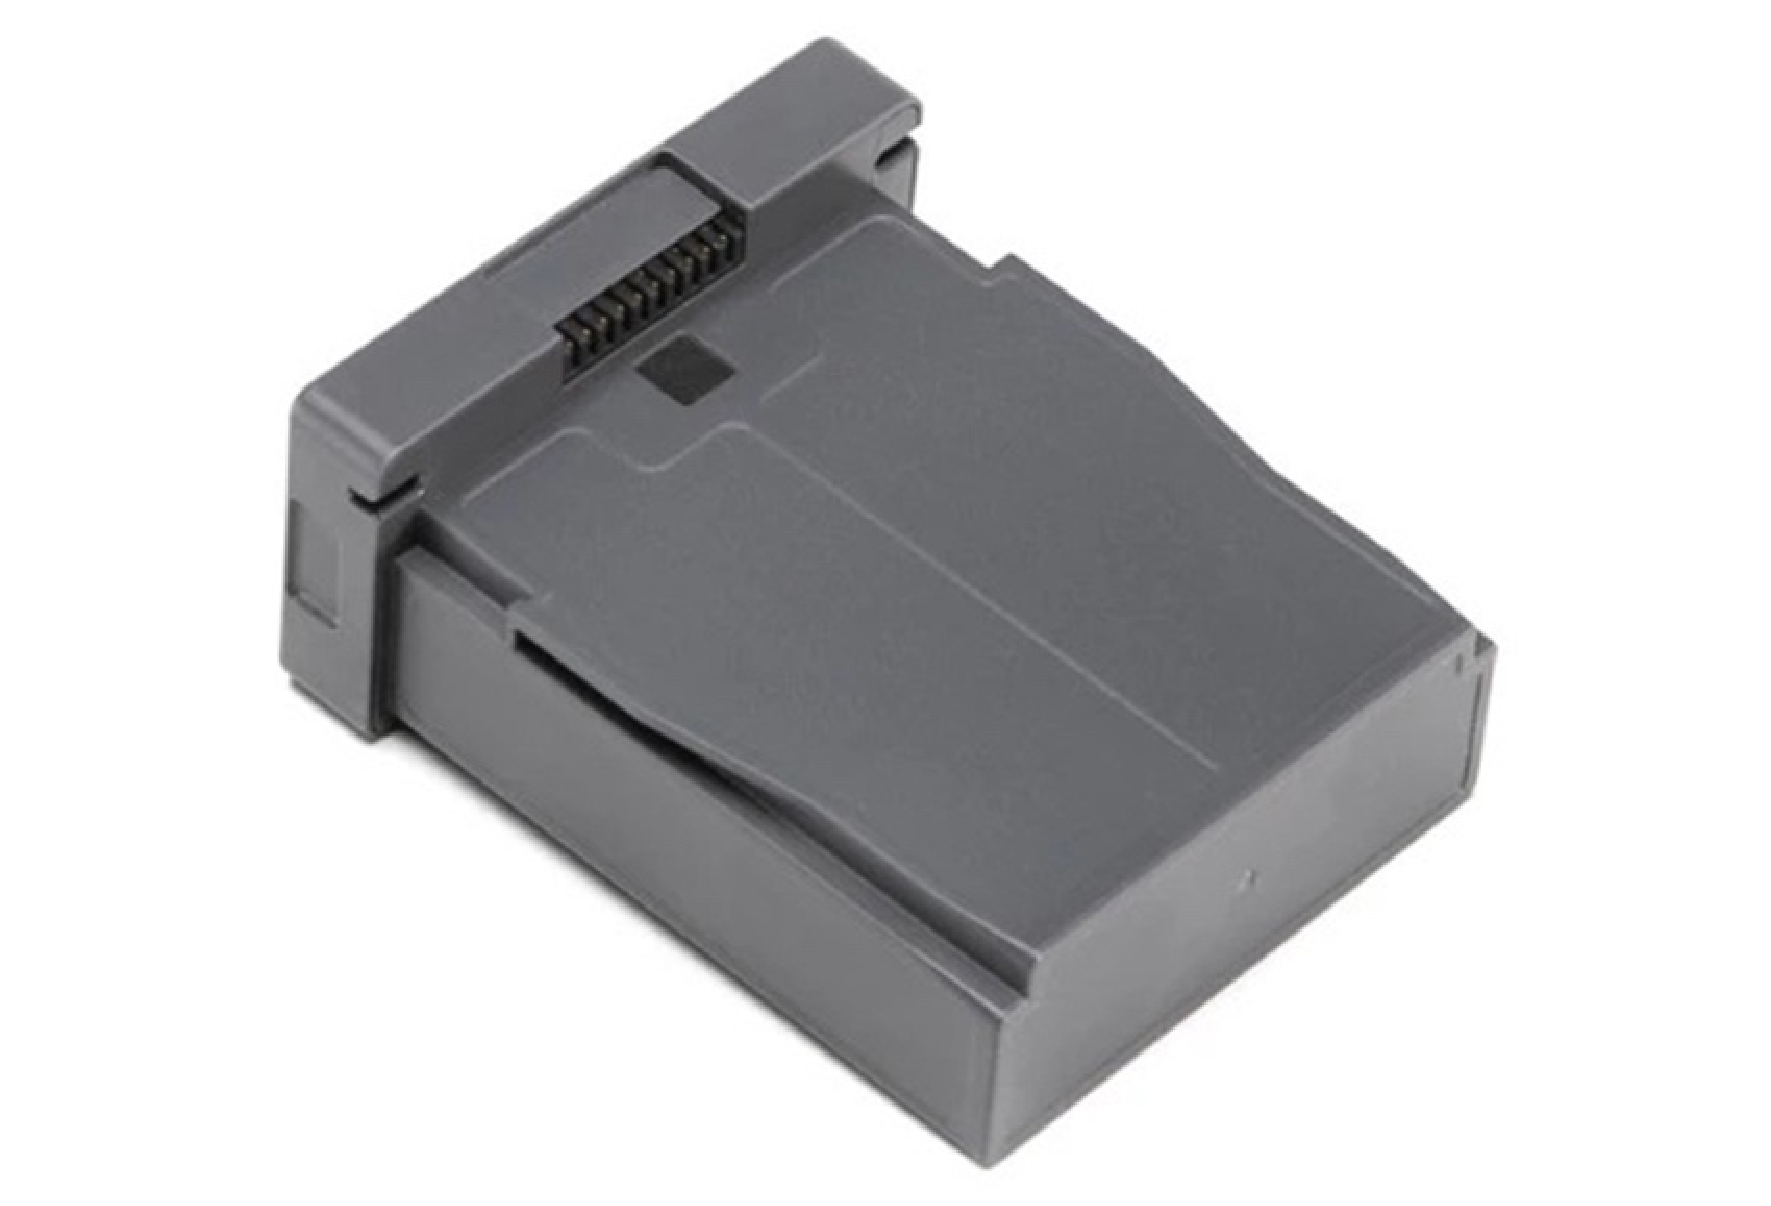
\includegraphics[width=\linewidth]{figures/fig_ep_battery.pdf}
    \end{minipage}
    \hfill
    \begin{minipage}{0.48\textwidth}
      \centering
      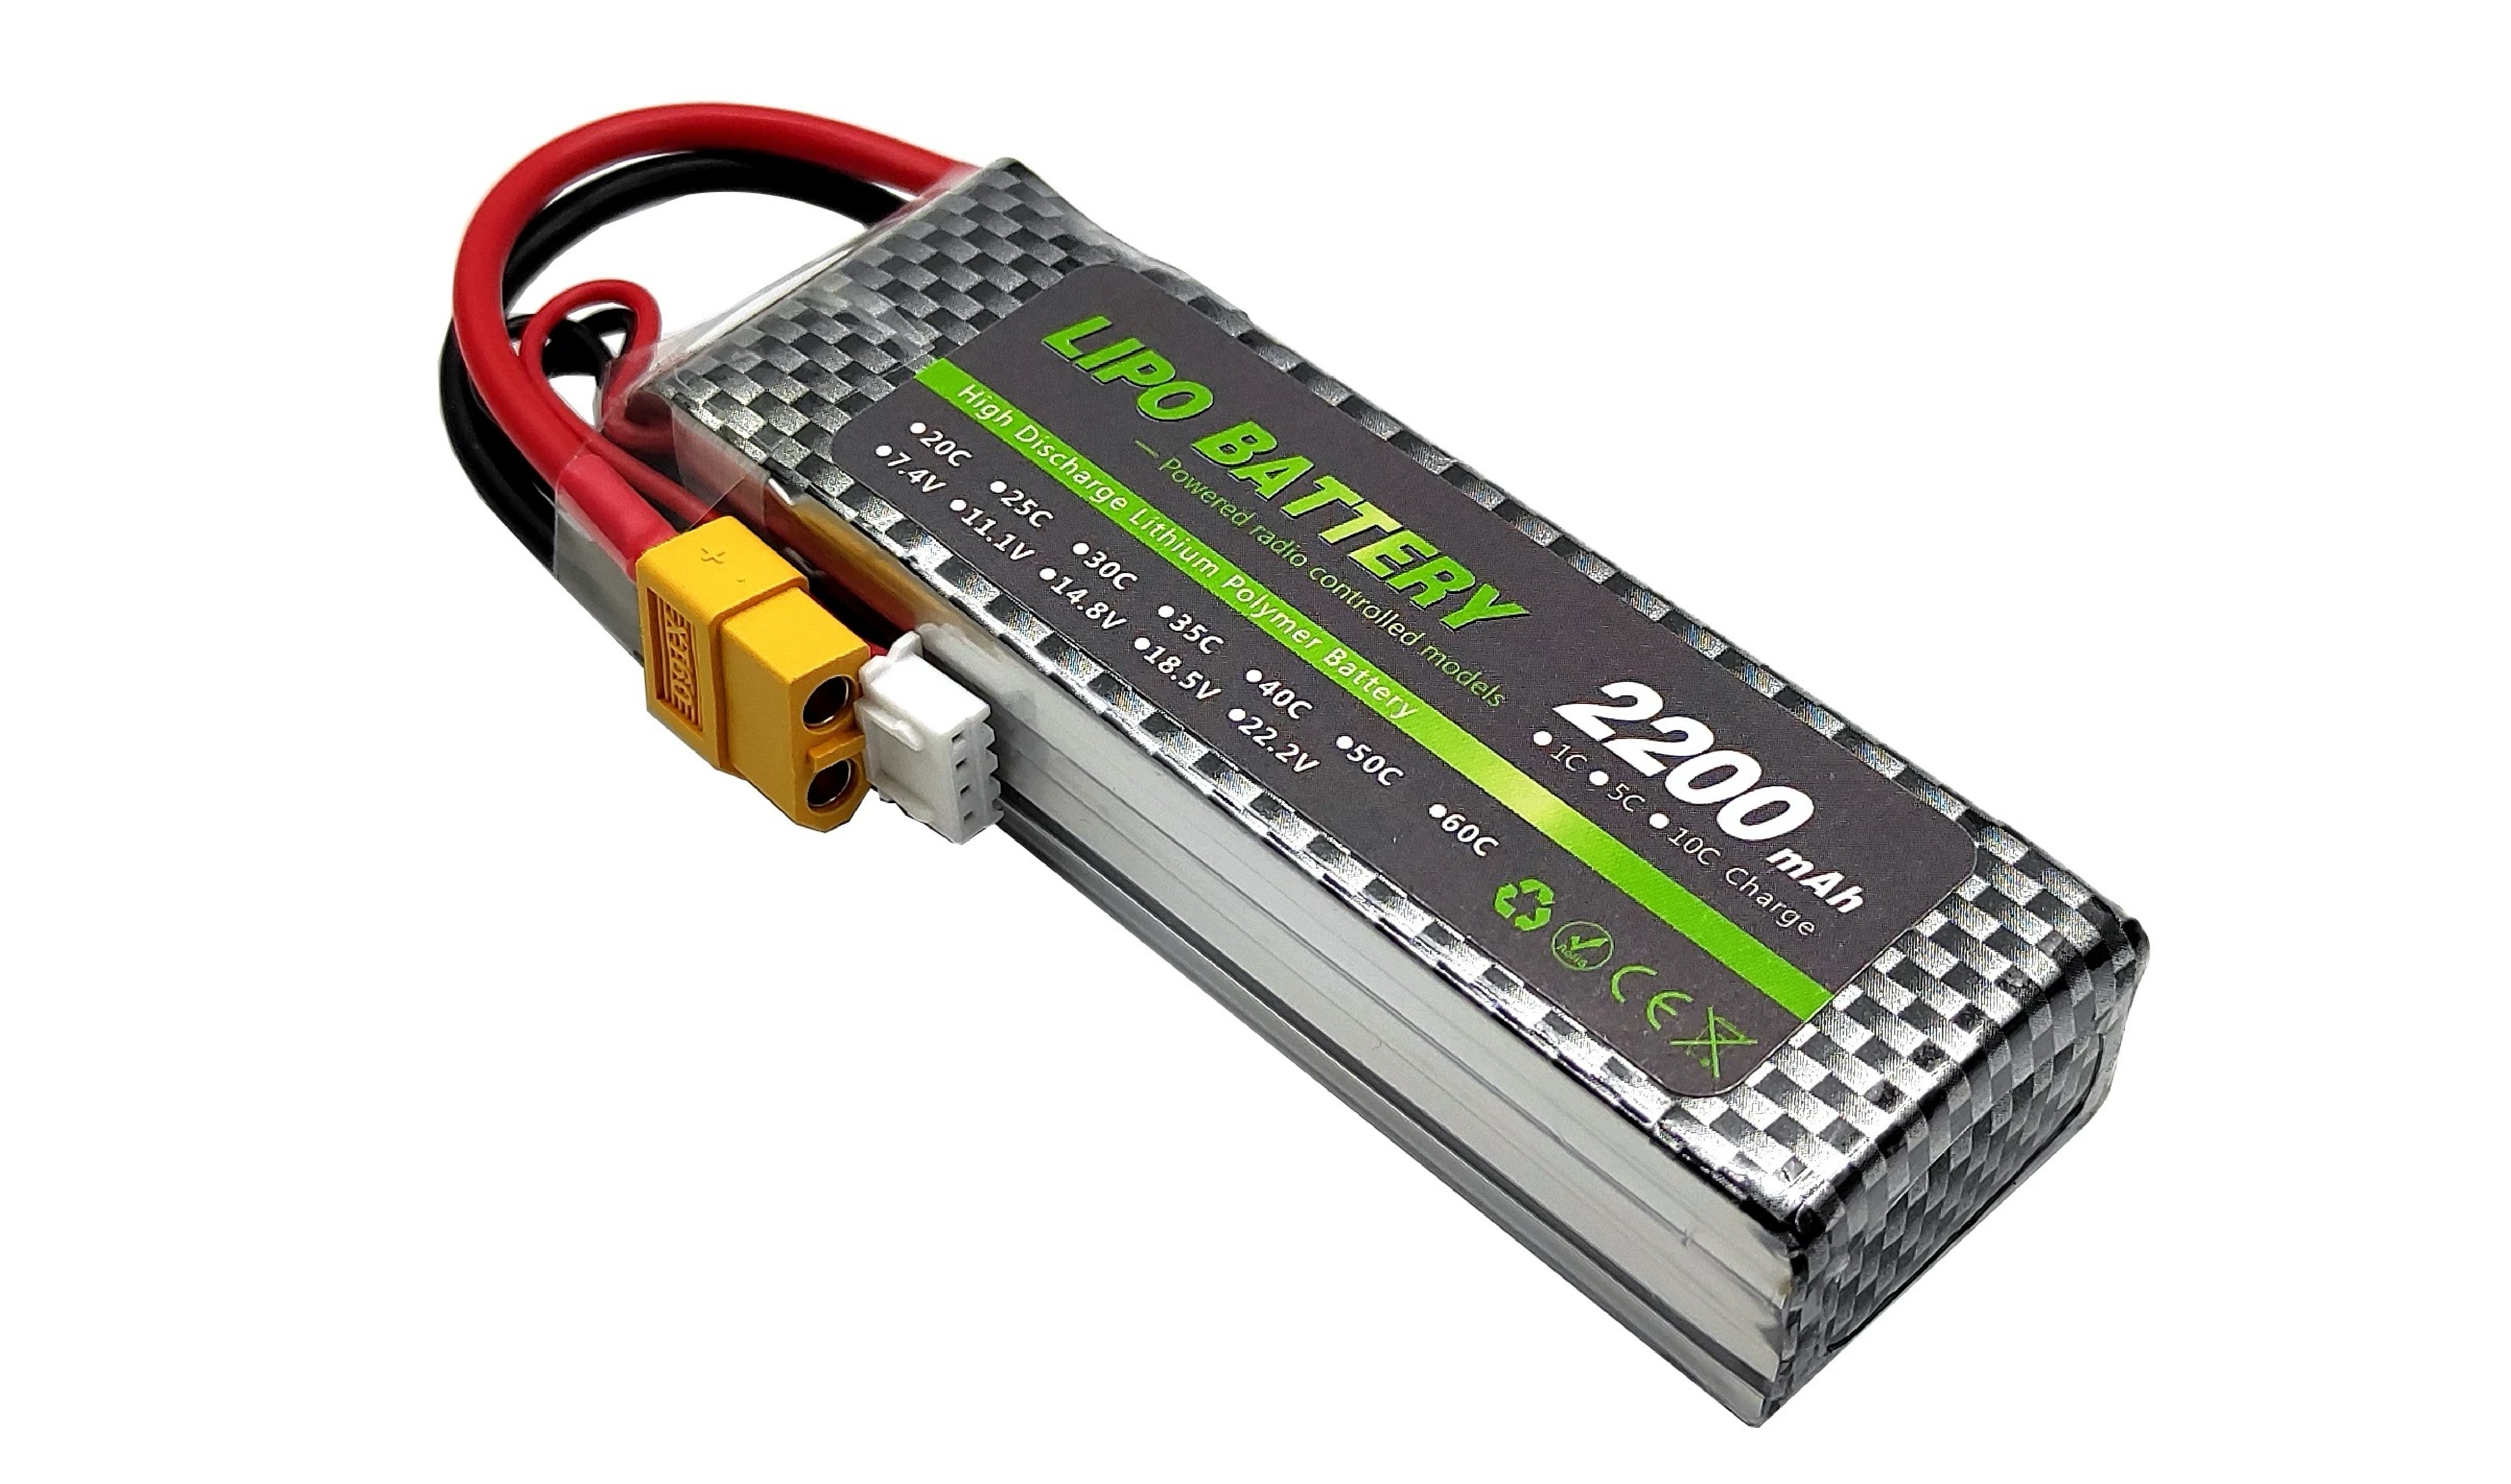
\includegraphics[width=\linewidth]{figures/fig_motor_battery.pdf}
    \end{minipage}
    \label{fig_ep_battery}
    \caption{A physical picture of Robomaster EP battery \& Motor-driven 3S LiPo battery.}
  \end{figure}

  \item \textbf{Logic Power:} The Jetson Orin NX requires a stable 19V input. To prevent logic resets caused by motor back-EMF, it is powered by a galvanically isolated power source.
  \item \textbf{Common Grounding:} Crucially, the ground (GND) planes of the Jetson Orin NX and the BTS7960 motor drivers are tied together to ensure reliable logic-level signal transmission.
\end{itemize}